\chapter{Laporan Database}
\section{Membuat Aplikasi Dari Data Excel}
\par
\begin{enumerate}
    \item Kunjungi Aplikasi APEX \textit{https://apex.oracle.com/} 
    \item Kemudian Masuk pada APEX nya dengan Melakukan \textit{SIGN IN} jika tidak memiliki akun maka lakukan \textit{SIGN UP}.
    \item Lalu jika sudah masuk Aplikasi APEX nya maka akan muncul seperti gambar dibawah.
    \begin{figure}[!htbp]
\centering
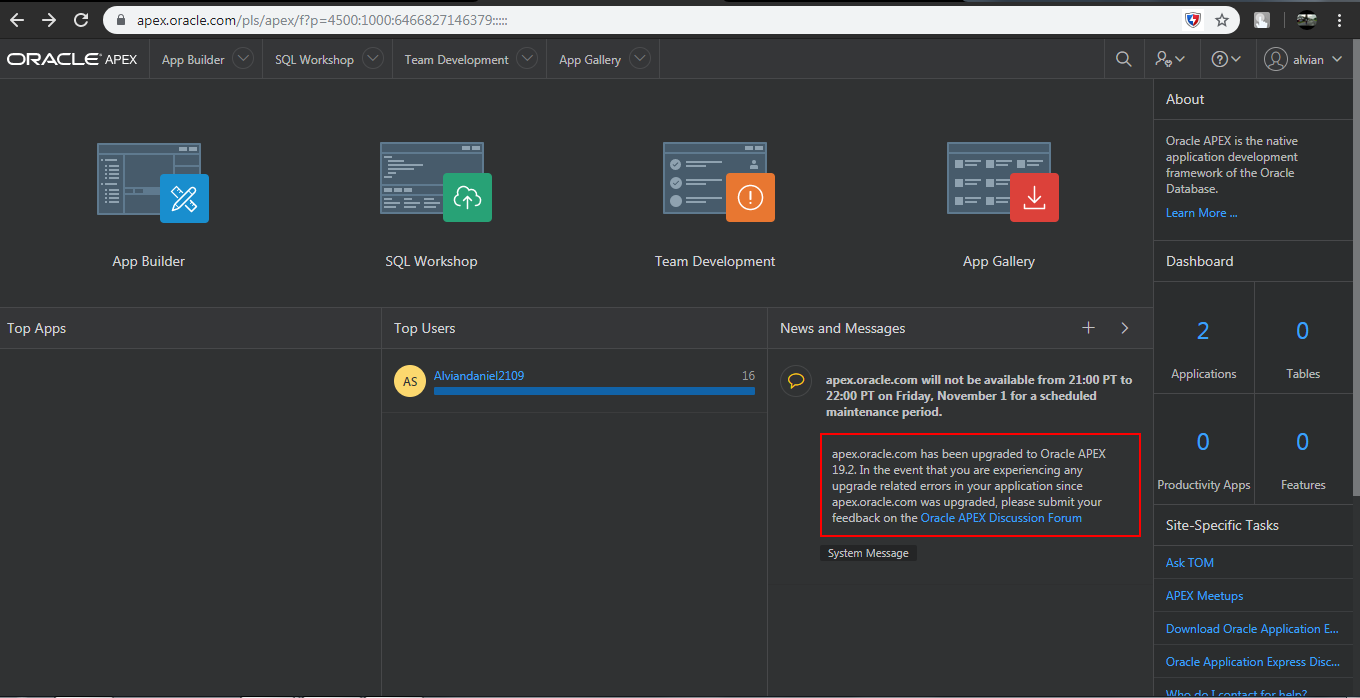
\includegraphics[width=10cm,height=9cm]{figures/A.PNG}
\caption{Menu Awal}
\label{penanda}
\end{figure}
    \item Kemudian Masuk Ke \textit{APP BUILDER}.
\begin{figure}[!htbp]
\centering
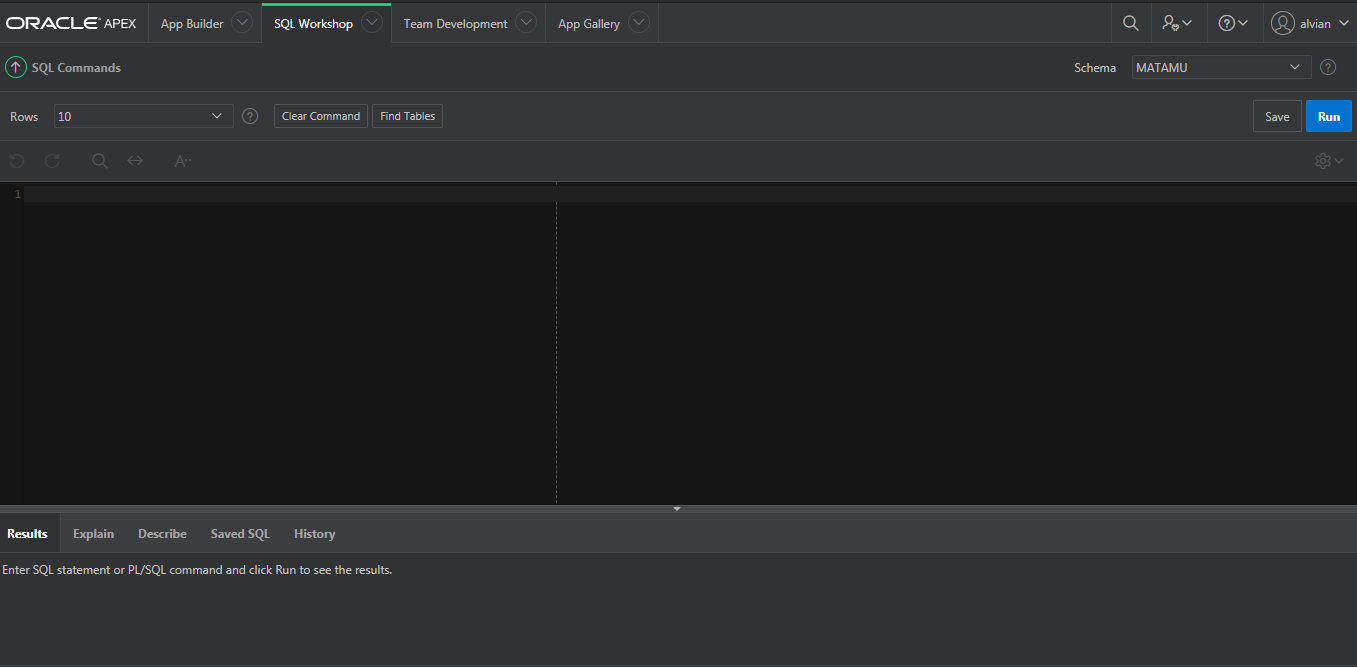
\includegraphics[width=11cm,height=9cm]{figures/B.PNG}
\caption{Menu APP BUILDER}
\label{penanda}
\end{figure}
    \item Masuk ke Halaman \textbf{Create}
\begin{figure}[!htbp]
\centering
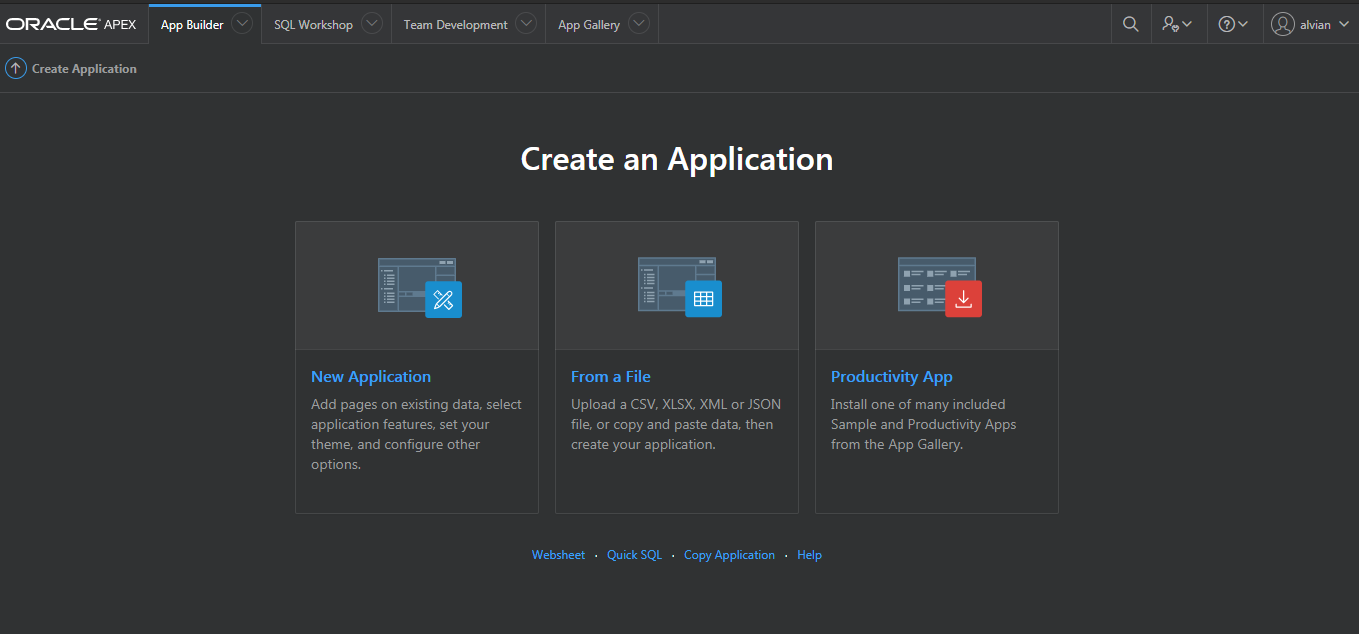
\includegraphics[width=11cm,height=9cm]{figures/C.PNG}
\caption{Menu Create}
\label{penanda}
\end{figure}
    \item Jika sudah maka Klik \textit{From a file}
\begin{figure}[!htbp]
\centering
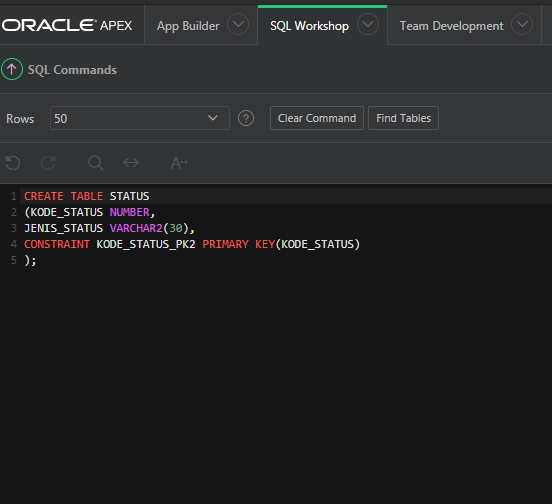
\includegraphics[width=10cm,height=8cm]{figures/D.PNG}
\caption{From a file}
\label{penanda}
\end{figure}
\item Kemudian Masukkan data yang sudah dinormalisasi dalam bentuk xlsx atau csv, disini saya memasukkan data yang sudah ada pada database 1 yaitu\textit{Data Mahasiswa} 
\item Akan muncul gambar seperti dibawah ini.
\begin{figure}[!htbp]
\centering
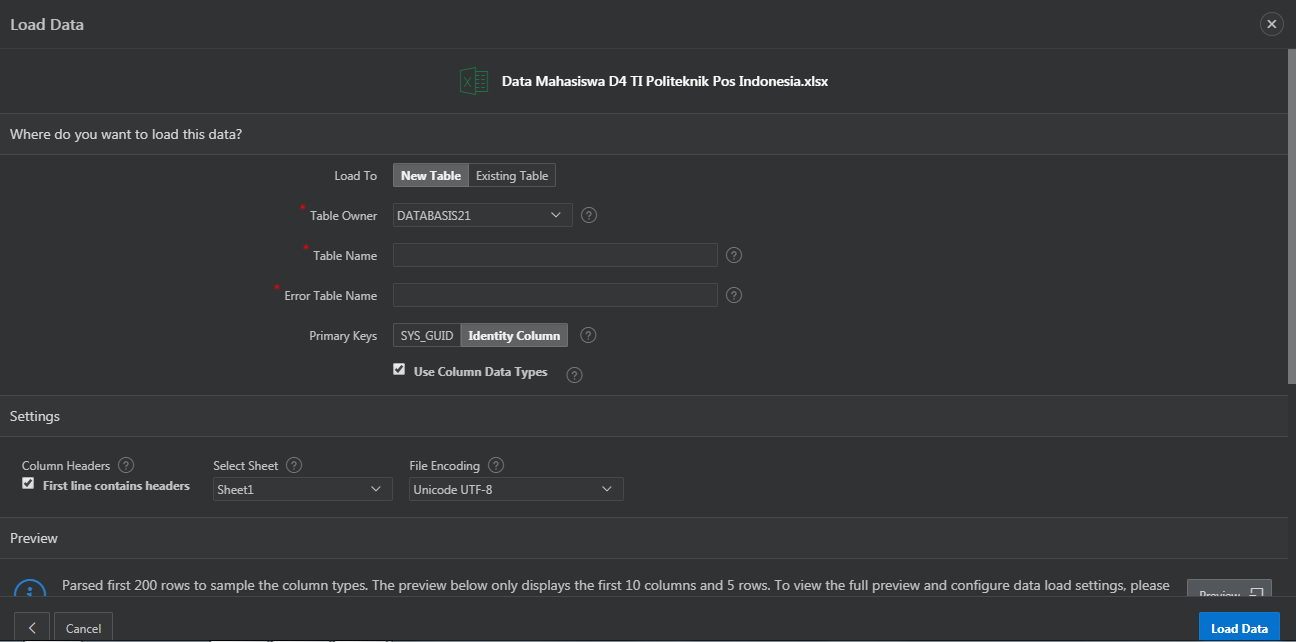
\includegraphics[width=10cm,height=7cm]{figures/E.PNG}
\caption{Upload File Excel}
\label{penanda}
\end{figure}
\item Pilih Tabel pada yang ingin diiputkan dengan memilih di \textbf{Select Sheet} Lalu Masukkan \textbf{Nama Table,}.
\begin{figure}[!htbp]
\centering
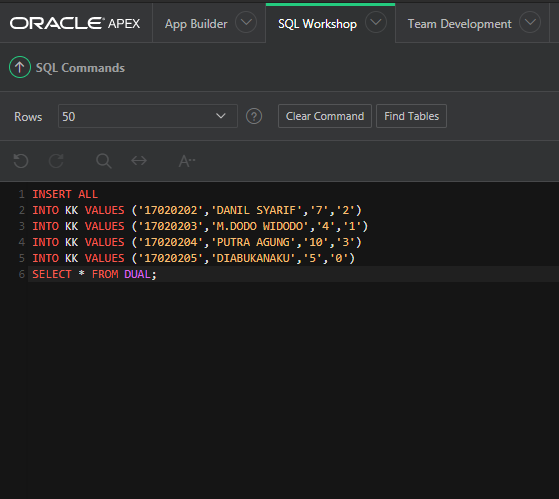
\includegraphics[width=10cm,height=8cm]{figures/F.PNG}
\caption{Save Changes}
\label{penanda}
\end{figure}
\item Jika Sudah tekan Configure pada bagian bawah Name table, Kemudian Save Change Seperti Gambar 1.7
\begin{figure}[!htbp]
\centering
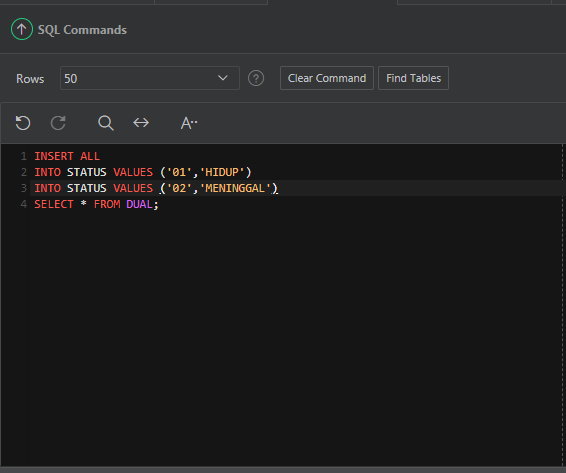
\includegraphics[width=11cm,height=7cm]{figures/F1.PNG}
\caption{Save Changes}
\label{penanda}
\end{figure}
\item Tekan Load Data.
\begin{figure}[!htbp]
\centering
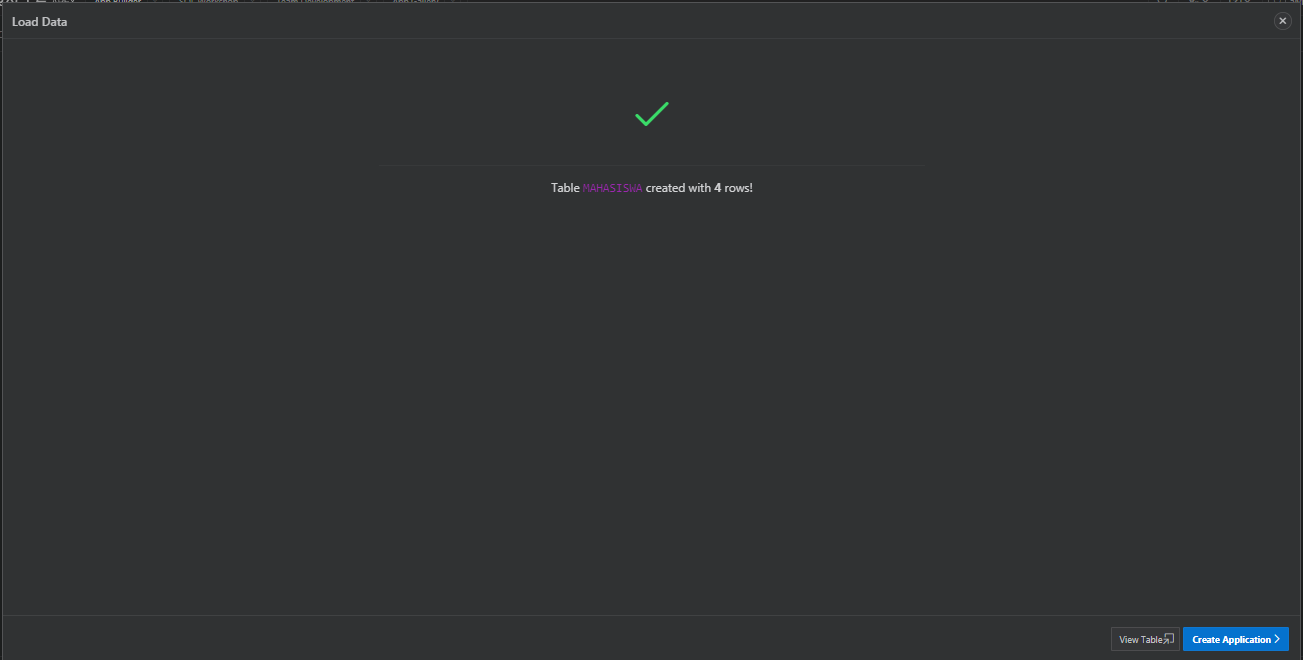
\includegraphics[width=11cm,height=8cm]{figures/G1.PNG}
\caption{load Data}
\label{penanda}
\end{figure}
\item Disini, ada 4 rows yang artinya ada 4 record data masuk pada data tersebut.
\item  Lakukan dengan cara yang sama dari tahap 5 hingga tahap 11 sesuai tabel yang diupload.
\item  Jika sudah setelah itu kita akan melakukan penghapusan kolom ID, ini dikarenakan ID diberikan otomatis oleh sistem apex jika di file kita tidak memiliki primary key.
\item Masuk ke Sql Workshop dan klik object browser.
\begin{figure}[!htbp]
\centering
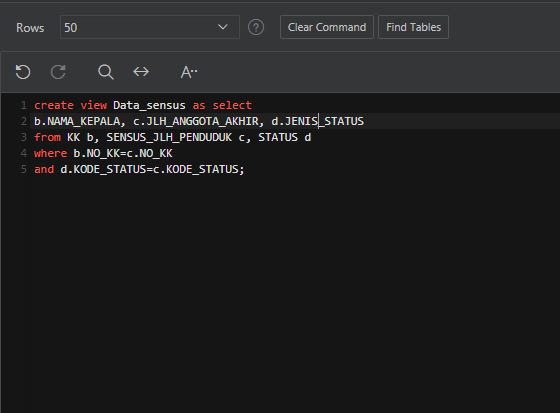
\includegraphics[width=10cm,height=7cm]{figures/H1.PNG}
\caption{Klik Object Browser}
\label{penanda}
\end{figure}
\item Selanjutnya kita klik tabel yang ingin kita drop disini saya menggunakan tabel \textbf{MAHASISWA}, Contoh seperti gambar 1.10 dibawah ini.
\begin{figure}[!htbp]
\centering
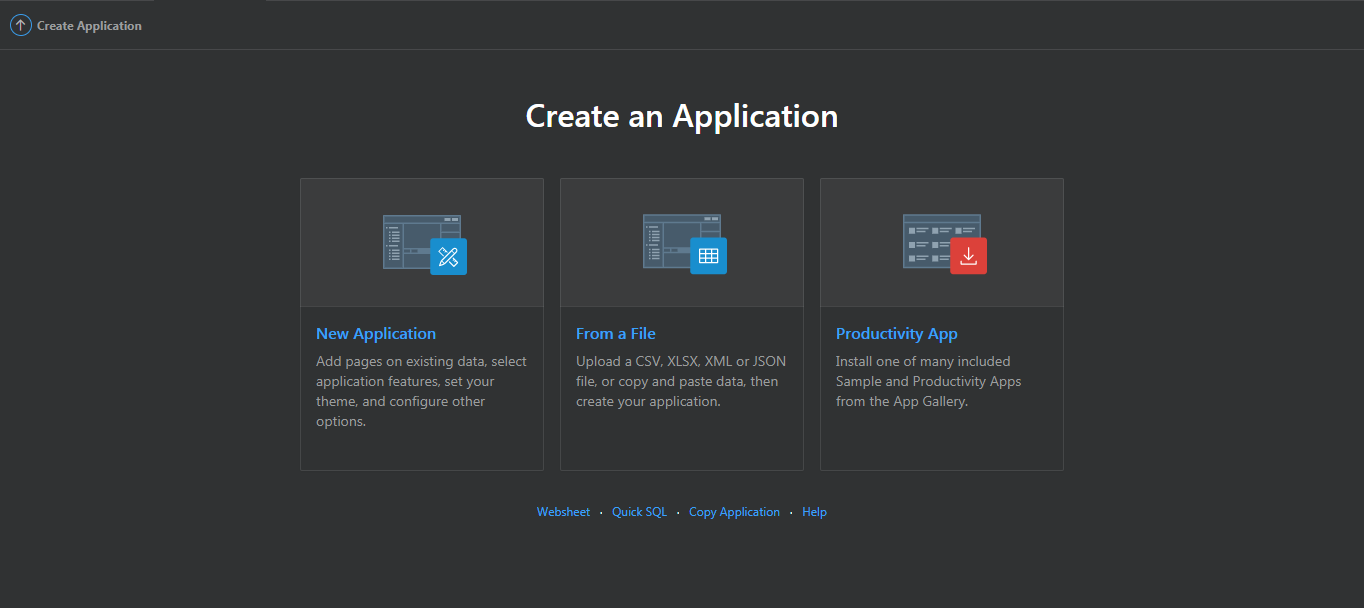
\includegraphics[width=10cm,height=7cm]{figures/H2.PNG}
\caption{Pilih Table yang ingin di drop column nya}
\label{penanda}
\end{figure}
\item Jika sudah, klik Drop Column lalu pilih kolom yang ingin di drop klik drop, Lalu klik finish lakukan berulang hingga semua tabel terbebas dari primary key.
\item Setelah itu kita akan add primary key kesetiap tabel yang telah kita upload.
\item Masuk ke sql Workshop dan klik Sql commands, Lalu ketik perintah seperti gambar dibawah ini.
\begin{figure}[!htbp]
\centering
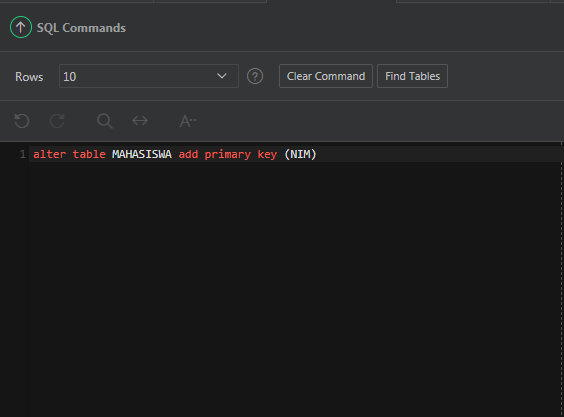
\includegraphics[width=10cm,height=7cm]{figures/H3.PNG}
\caption{Membuat Primary key Setiap tabel}
\label{penanda}
\end{figure}
\item Setelah itu kita run, tunggu hingga muncul pesan table altered.
\item Langkah selanjutnya adalah cara merelasikan dua tabel, yaitu kita mengketikkan query seperti gambar dibawah.
\begin{figure}[!htbp]
\centering
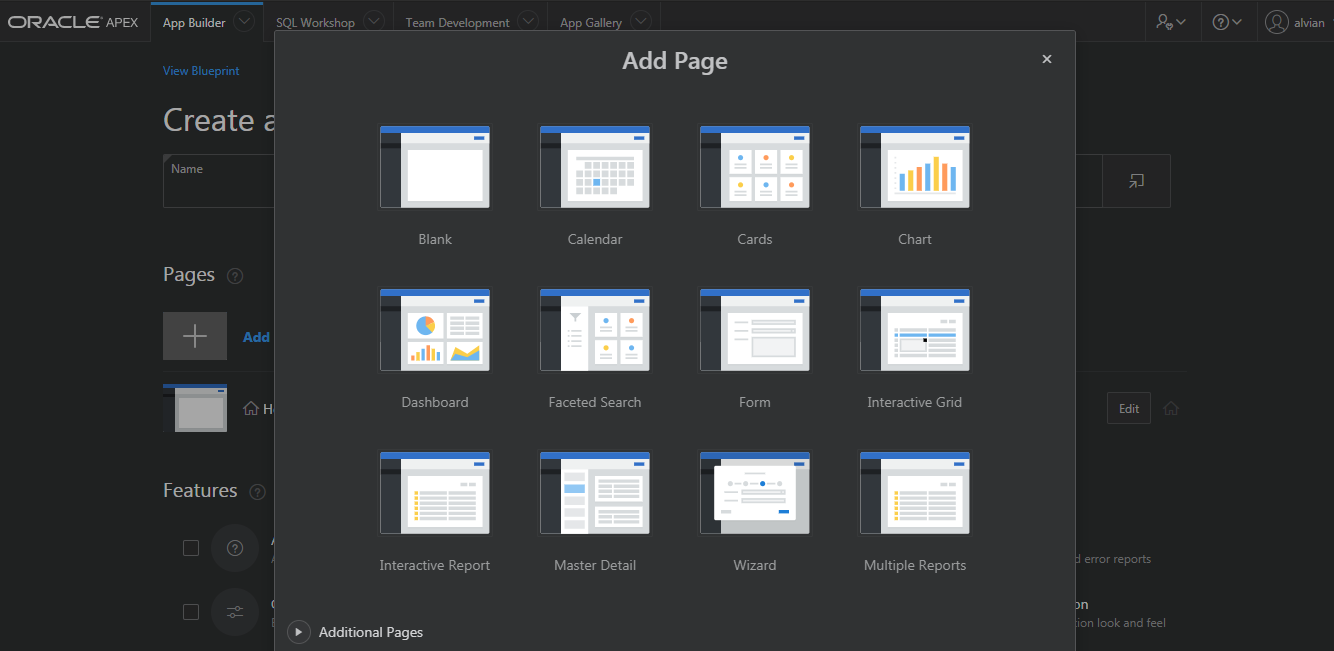
\includegraphics[width=10cm,height=7cm]{figures/H4.PNG}
\caption{Menambahkan Foreign key pada tabel yang berelasi}
\label{penanda}
\end{figure}
\item untuk melihat Relasi antar tabel dapat meliha pada \textbf{MODEL}
\item Langkah selanjutnya kita ke app builder lalu klik create lalu klik new application.
\begin{figure}[!htbp]
\centering
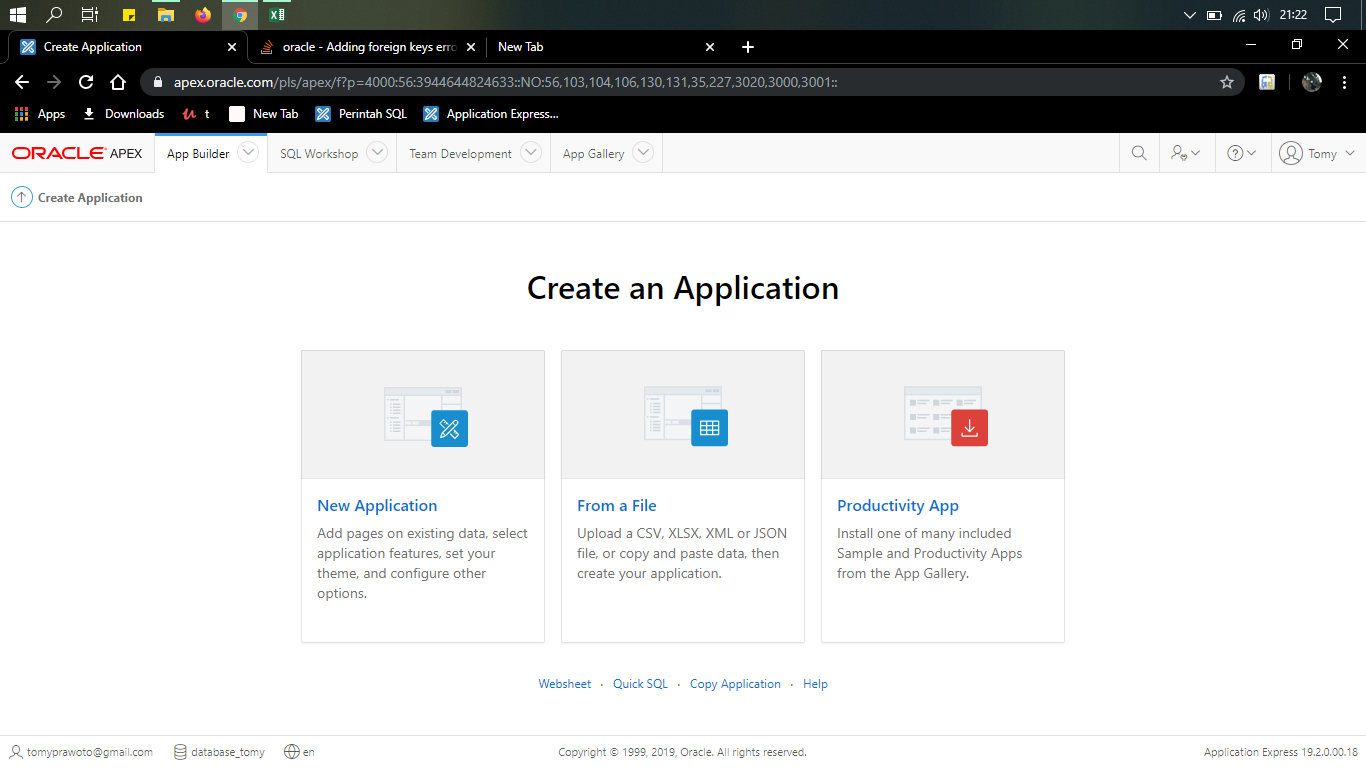
\includegraphics[width=10cm,height=7cm]{figures/H5.PNG}
\caption{Create Applications}
\label{penanda}
\end{figure}
\item  Setelah itu add page.
\begin{figure}[!htbp]
\centering
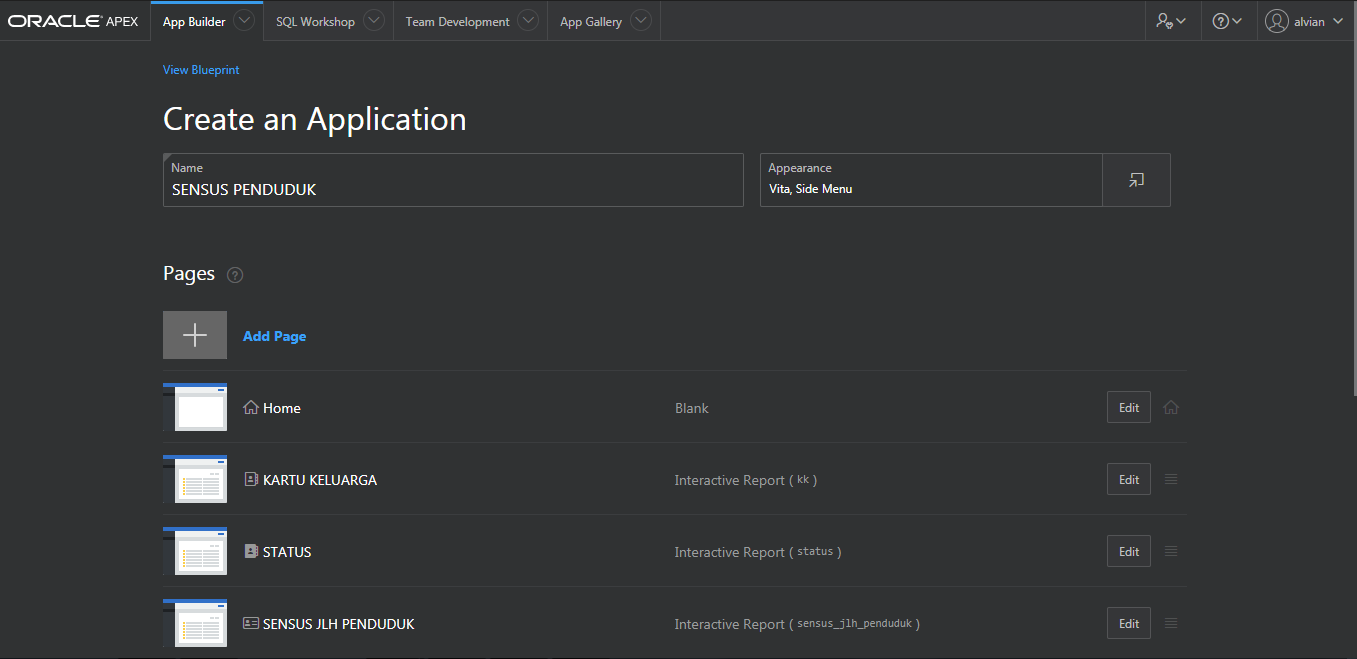
\includegraphics[width=10cm,height=7cm]{figures/H6.PNG}
\caption{Add page}
\label{penanda}
\end{figure}
\item Kita pilih interactive report.
\item Kemudian pilih tabel dan Beri nama.
\begin{figure}[!htbp]
\centering
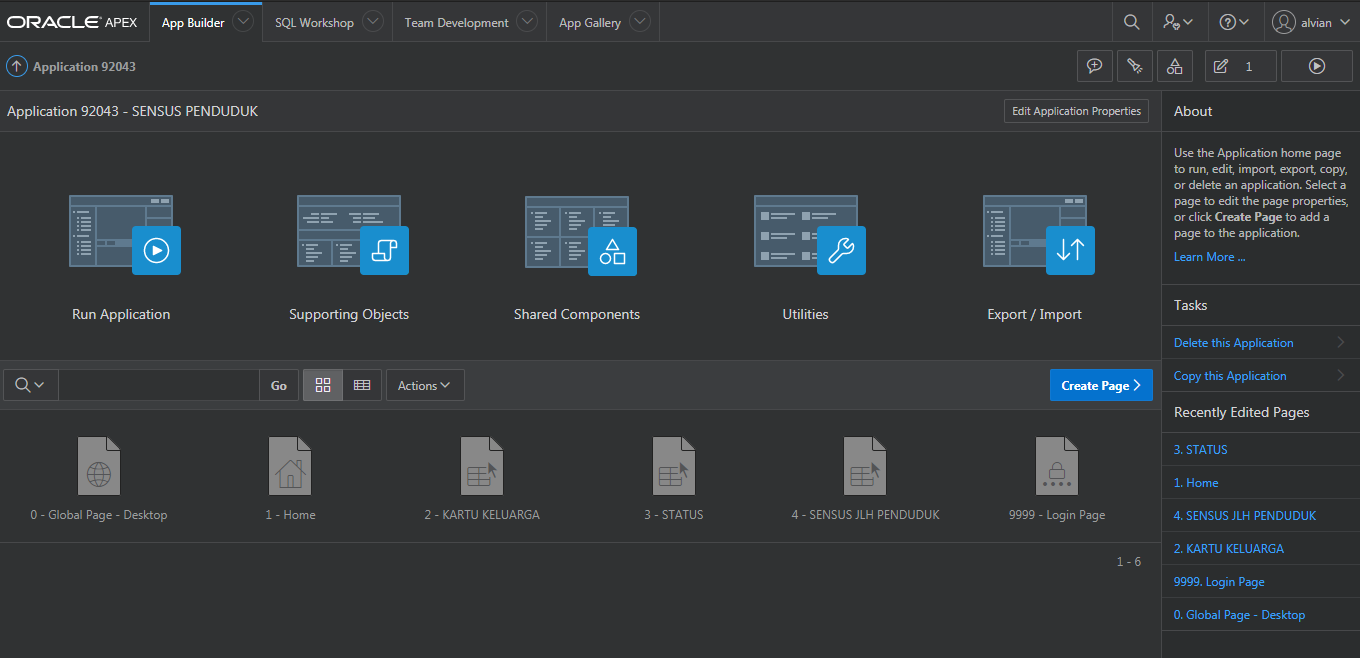
\includegraphics[width=10cm,height=7cm]{figures/H7.PNG}
\caption{Beri Nama Add Page}
\label{penanda}
\end{figure}
\item Ulangi Step diatas sampai semua tabel masuk.
\item  Scroll kebawah lalu klik create application.
\item Run application.
\begin{figure}[!htbp]
\centering
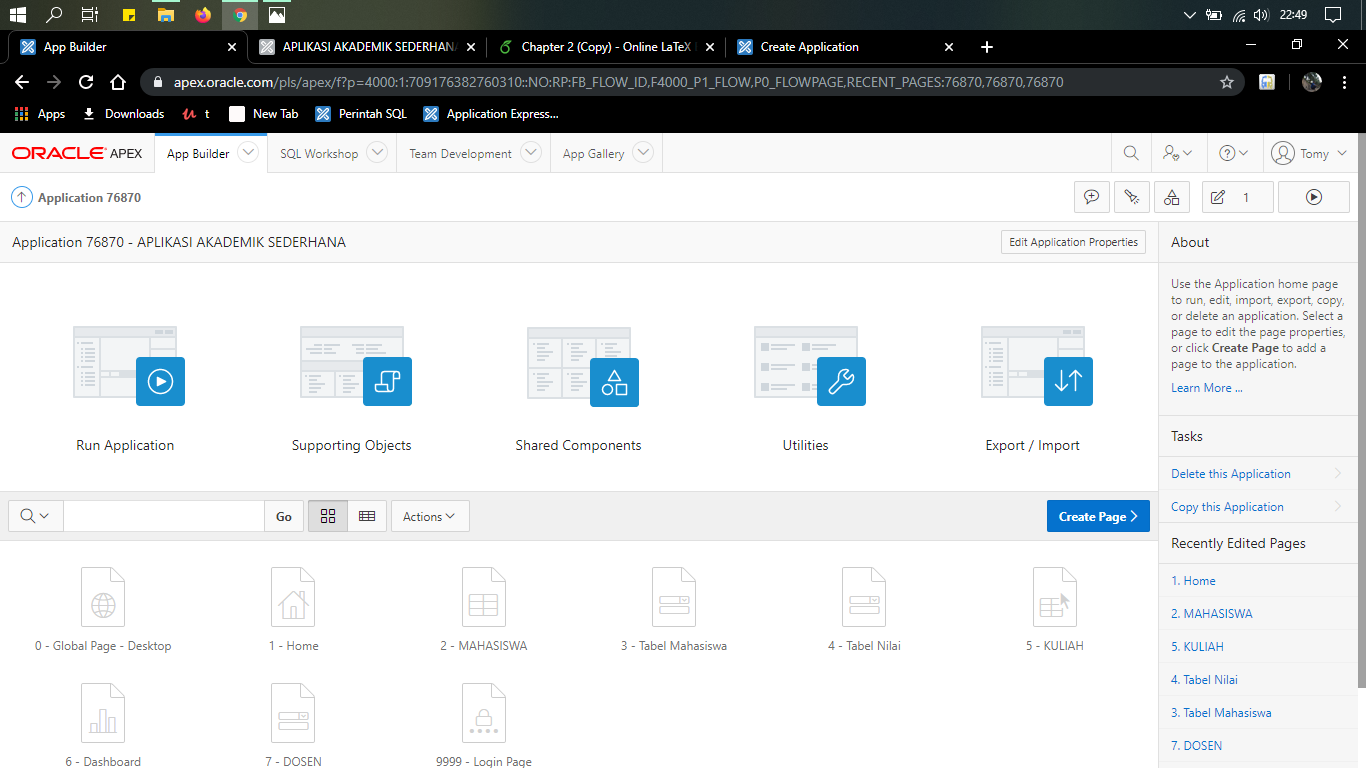
\includegraphics[width=10cm,height=8.5cm]{figures/H8.PNG}
\caption{run application}\\
\label{penanda}
\end{figure}
\item Nah telah selesai.
\begin{figure}[!htbp]
\centering
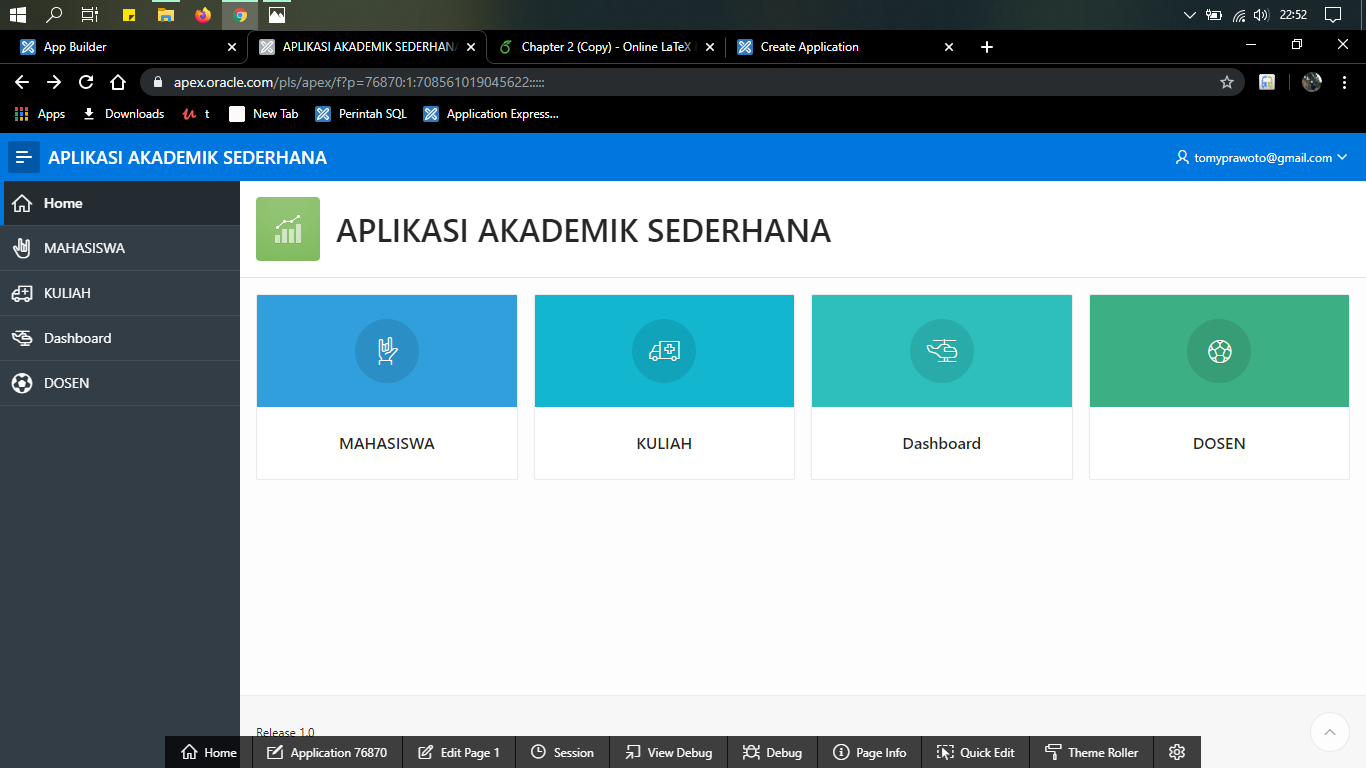
\includegraphics[width=10cm,height=7cm]{figures/H9.PNG}
\caption{run application}
\label{penanda}
\end{figure}
\end{enumerate}

